%----------------------------------------------------------------------------------------
%	SOLUTION 2.a
%----------------------------------------------------------------------------------------
\subsection*{Solution 2.a}
\begin{figure}[h!]
	\centering
	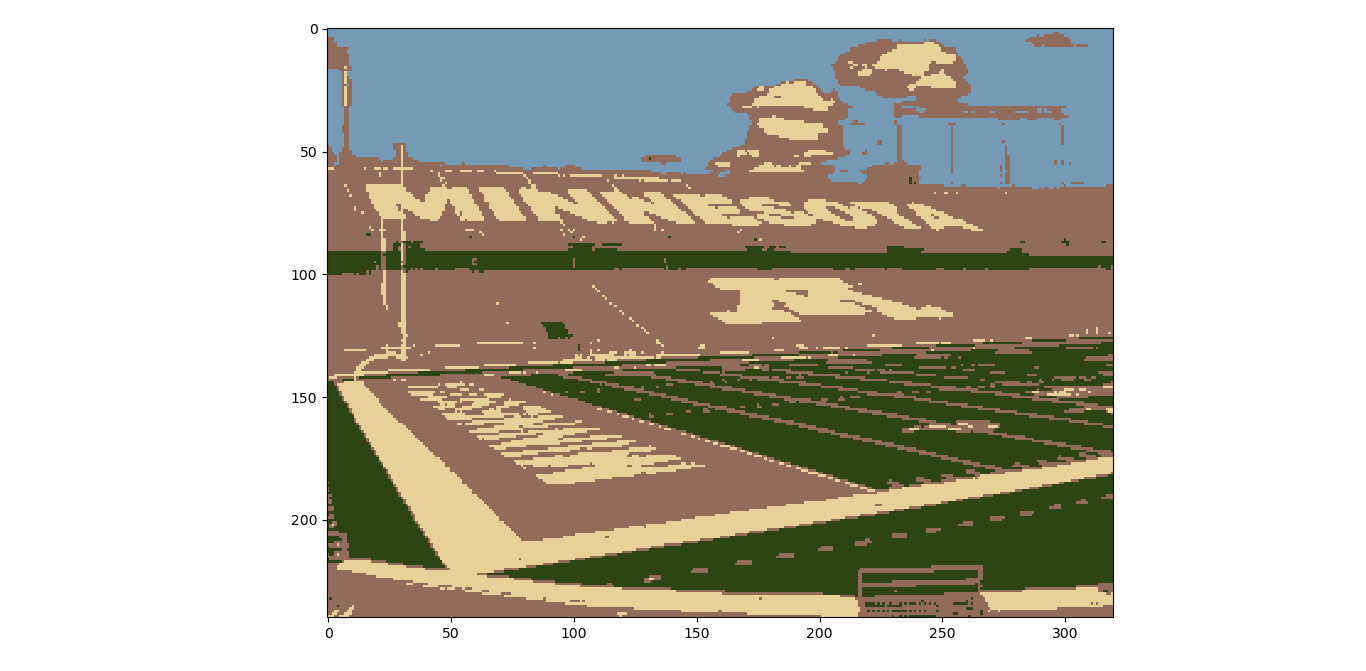
\includegraphics[scale=0.5]{q2_a_k_4}
	\caption{Q2.a: EM on 'stadium.jpg' with k=4 and 200 iterations}
	\label{fig:2a_em_4}
\end{figure}
\begin{figure}[h!]
	\centering
	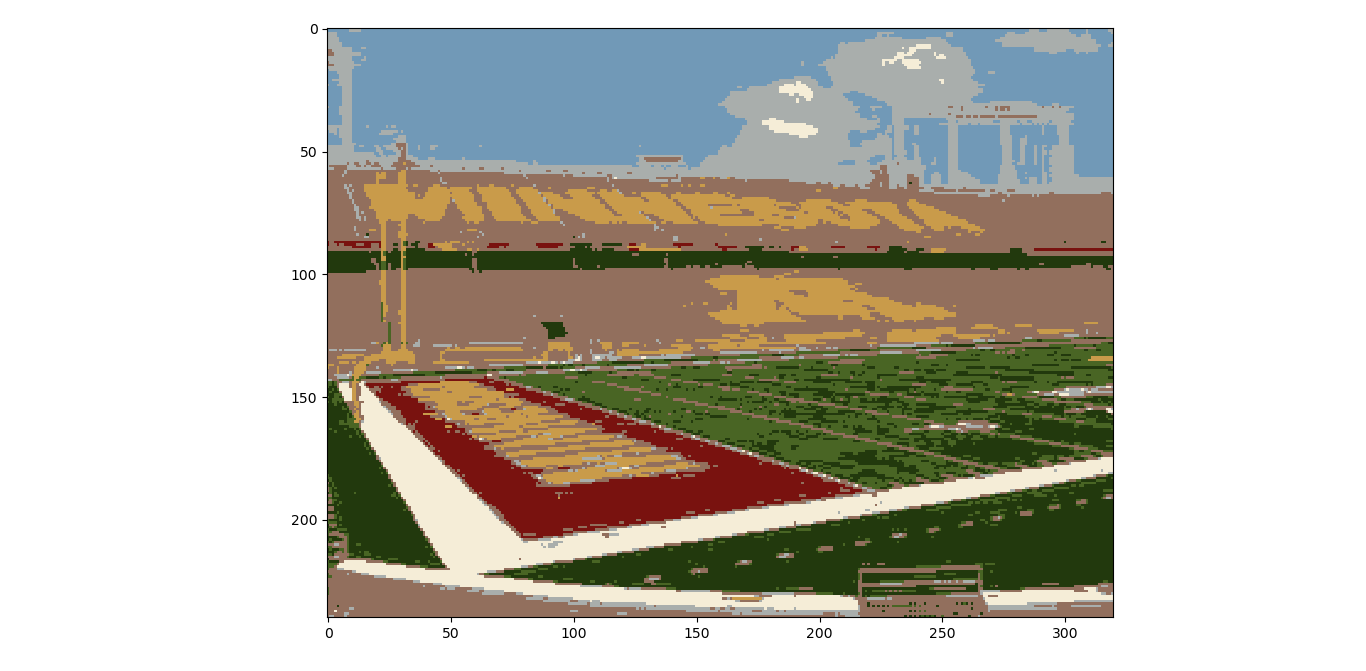
\includegraphics[scale=0.5]{q2_a_k_8}
	\caption{Q2.a: EM on 'stadium.jpg' with k=8 and 200 iterations}
	\label{fig:2a_em_8}
\end{figure}
\begin{figure}[h!]
	\centering
	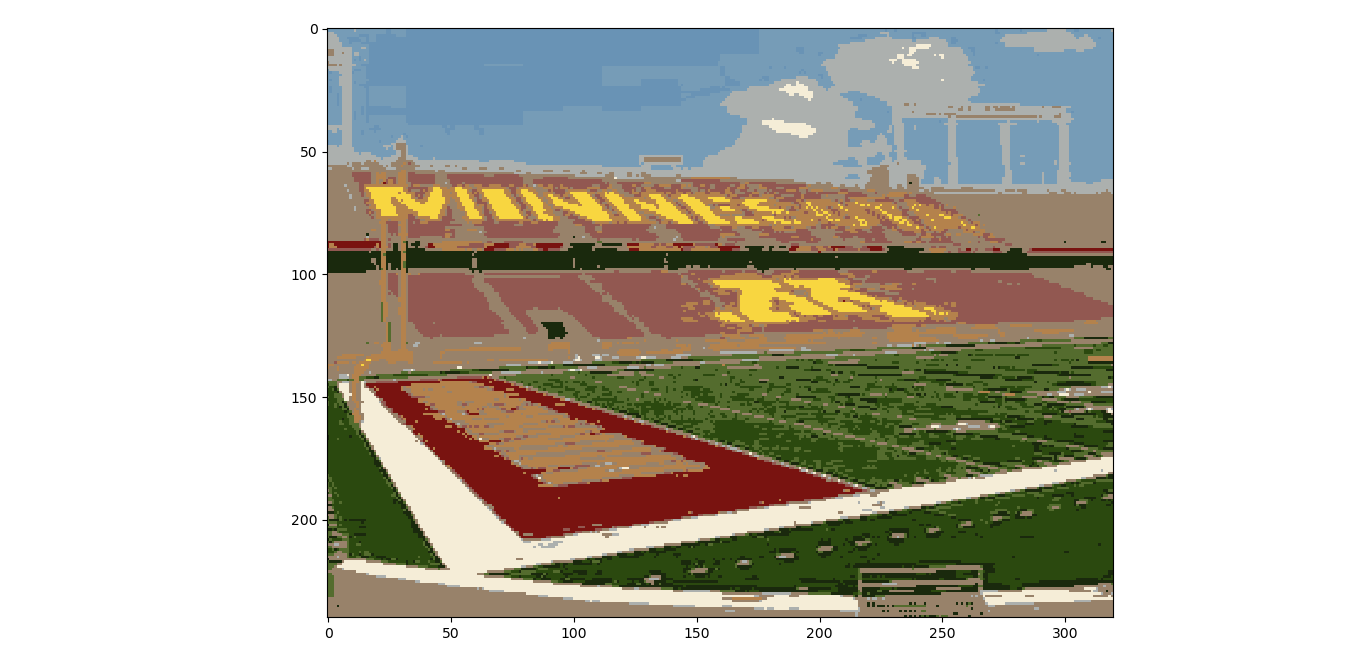
\includegraphics[scale=0.5]{q2_a_k_12}
	\caption{Q2.a: EM on 'stadium.jpg' with k=12 and 200 iterations}
	\label{fig:2a_em_12}
\end{figure}
\newpage
\subsection*{Solution 2.b}
\begin{figure}[h!]
	\centering
	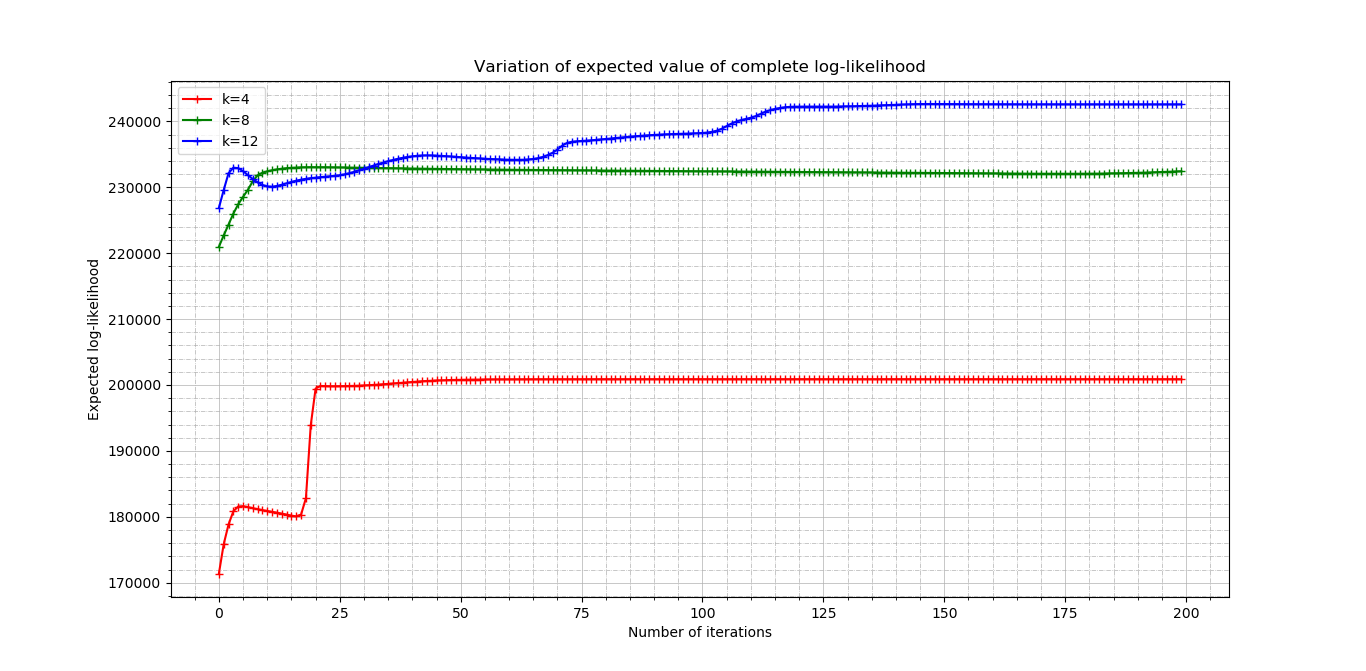
\includegraphics[scale=0.5]{q2_b_exp_llh}
	\caption{Q2.b: Expected value of log-likelihood on 'stadium.jpg' with different k}
	\label{fig:2b_em_llh}
\end{figure}
It can be seen from Fig.~\ref{fig:2b_em_llh} that for each single value of k, expected value of complete log-likelihood gets maximized and after a certain iteration it does not increase any more which denotes convergence. Moreover, as the value of k increases, expected value of complete log-likelihood also increases which means higher the value of k, the image becomes closer to original one. Though it reduces compression ratio but gives higher quality picture.
\subsection*{Solution 2.c}
Trying to run EM algorithm on 'goldy.jpg' raises runtime error while calculating $P(\xVec^t|\phi)$ as the covariance matrix becomes singular. Therefore, as the inverse of the covariance matrix cannot be calculated, we cannot calculate gaussian pdf value and cannot proceed further with E-step.
\begin{figure}[h!]
	\centering
	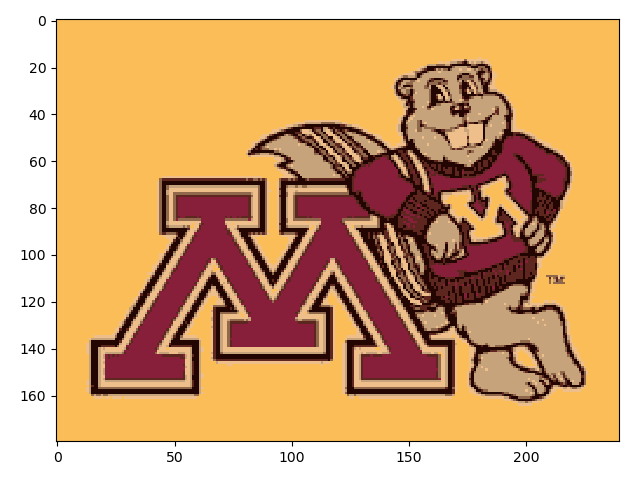
\includegraphics[scale=0.5]{q2_c_goldy_kmeans}
	\caption{Q2.c: K-means on 'goldy.jpg'}
	\label{fig:2c_goldy}
\end{figure}
Fig.~(\ref{fig:2c_goldy}) shows the result after compression of 'goldy.jpg' with k-means algorithm. The behavior of k-means and EM algorithm differs significantly as k-means does not use any parametric methods whereas in EM, the approach is probabilistic and depends on finding the parameters of underlying mixture of assumed probability density functions. 
\newpage

%----------------------------------------------------------------------------------------
%	SOLUTION 2.d
%----------------------------------------------------------------------------------------
\subsection*{Solution 2.d}
In the M-step, To find the estimate of $\SigmaVec_i$ with regularization, first let us write the terms of expected complete log-likelihood function which depends on $\SigmaVec_i$ as the other terms will eventually become 0 when we will take the derivative. We will also use the fact that
\begin{equation*}
\xVec^T A \xVec = trace[\xVec^T A \xVec] = trace[\xVec \xVec^T A]
\end{equation*} 
The expectation of complete log-likelihood function involving the terms that depend on $\sVec_i$ can be written as:
\begin{equation}
\begin{split}
\mathcal{E}(\phi|\phi^l) &= \sum_{t=1}^{N} \sum_{i=1}^{K} h_i^t \ln p_i(\xVec^t|\phi^l) - \frac{\lambda}{2}\sum_{i=1}^{K} \sum_{j=1}^{d}\left(\SigmaVec_i^{-1}\right)_{jj}\\
&= \sum_{t=1}^{N} \sum_{i=1}^{K} h_i^t\left[-\frac{d}{2}\ln (2\pi) - \frac{1}{2}\ln |\SigmaVec_i| - \frac{1}{2}\left(\xVec^t-\mVec^{l+1}_i\right)^T \SigmaVec_i^{-1}\left(\xVec^t-\mVec^{l+1}_i\right)\right]-\frac{\lambda}{2} \sum_{i=1}^{K} \sum_{j=1}^{d}\left(\SigmaVec_i^{-1}\right)_{jj}\\
\end{split}
\end{equation}
Removing the $\ln(2\pi)$ term as it is independent of $\SigmaVec_i$, the above can be written as:
\begin{equation}
	\begin{split}
		\mathcal{E}'(\phi|\phi^l) &= \sum_{t=1}^{N} \sum_{i=1}^{K} \left[-\frac{h_i^t}{2}\ln|\SigmaVec_i| - \frac{h^t_i}{2}\left(trace\left((\xVec^t-\mVec^{l+1}_i)^T \SigmaVec_i^{-1}(\xVec^t-\mVec^{l+1}_i)\right)\right)\right]-\frac{\lambda}{2} \sum_{i=1}^{K} \sum_{j=1}^{d}\left(\SigmaVec_i^{-1}\right)_{jj}\\
		&= \sum_{t=1}^{N} \sum_{i=1}^{K} \left[-\frac{h_i^t}{2}\ln|\SigmaVec_i| - \frac{h^t_i}{2}\left(trace\left((\xVec^t-\mVec^{l+1}_i) (\xVec^t-\mVec^{l+1}_i)^T \SigmaVec_i^{-1}\right)\right)\right]-\frac{\lambda}{2} \sum_{i=1}^{K} \sum_{j=1}^{d}\left(\SigmaVec_i^{-1}\right)_{jj}\\
	\end{split}
\end{equation}
To find the estimate of $\SigmaVec_i$, what we denote as $\sVec^{l+1}_i$, we can equivalently set the derivative of $\mathcal{E}'(\phi|\phi^l)$ w.r.t $\SigmaVec_i^{-1}$ to 0, i.e.
\begin{equation}
\begin{split}
\frac{\partial \mathcal{E}'(\phi|\phi^l)}{\partial \SigmaVec_i^{-1}} &= 0\\
\implies & 0 = \sum_{t=1}^{N}h^t_i \sVec^{l+1}_i - \sum_{t=1}^{N}h^t_i(\xVec^t-\mVec^{l+1}_i)(\xVec^t-\mVec^{l+1}_i)^T-\frac{\lambda}{2}I\\
\implies & \sVec^{l+1}_i = \frac{\sum_{t=1}^{N} \left[h^t_i (\xVec^t-\mVec^{l+1}_i)(\xVec^t-\mVec^{l+1}_i)^T\right]+\frac{\lambda}{2}I}{\sum_{t=1}^{N}h^t_i}
\end{split}
\end{equation}
\newpage
\subsection*{Solution 2.e}
\begin{figure}[h!]
	\centering
	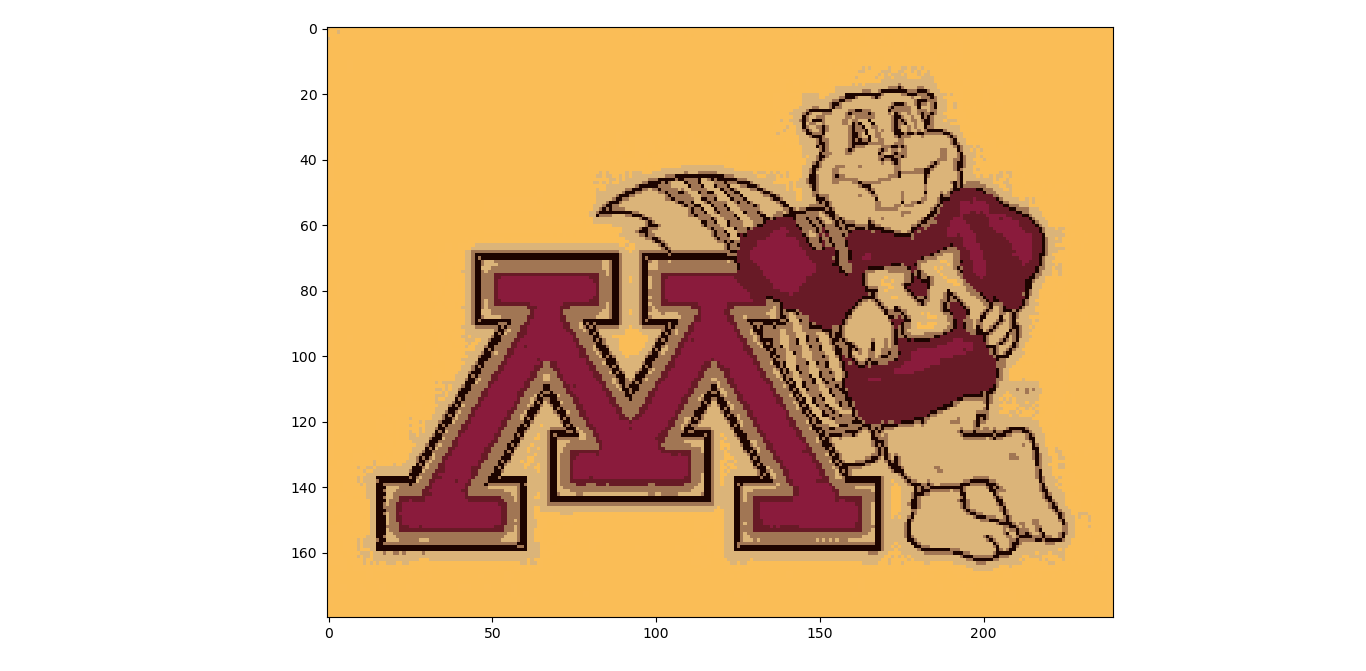
\includegraphics[scale=0.5]{q2_e_goldy_em}
	\caption{Q2.e: EM with regularization $\lambda = 0.0001$ on 'goldy.jpg' and 200 iterations}
	\label{fig:2e_goldy}
\end{figure}
When we add a regularization parameter, $\lambda = 0.0001$, the MLE of covariance matrix becomes non-singular as the regularization terms get added to the diagonal terms of covariance matrix. Therefore, we can see that the regularized EM can run the algorithm on 'goldy.jpg' and produces the Fig.~\ref{fig:2e_goldy}.